% ORES packages and the dependencies between them.
\documentclass{article}
\usepackage{tikz}
\usepackage[strict]{changepage}
\usepackage[a3paper]{geometry}
\usetikzlibrary{arrows,shapes}

% Disable page number for better SVG.
\pagenumbering{gobble}

\begin{document}
\begin{adjustwidth}{-7em}{}
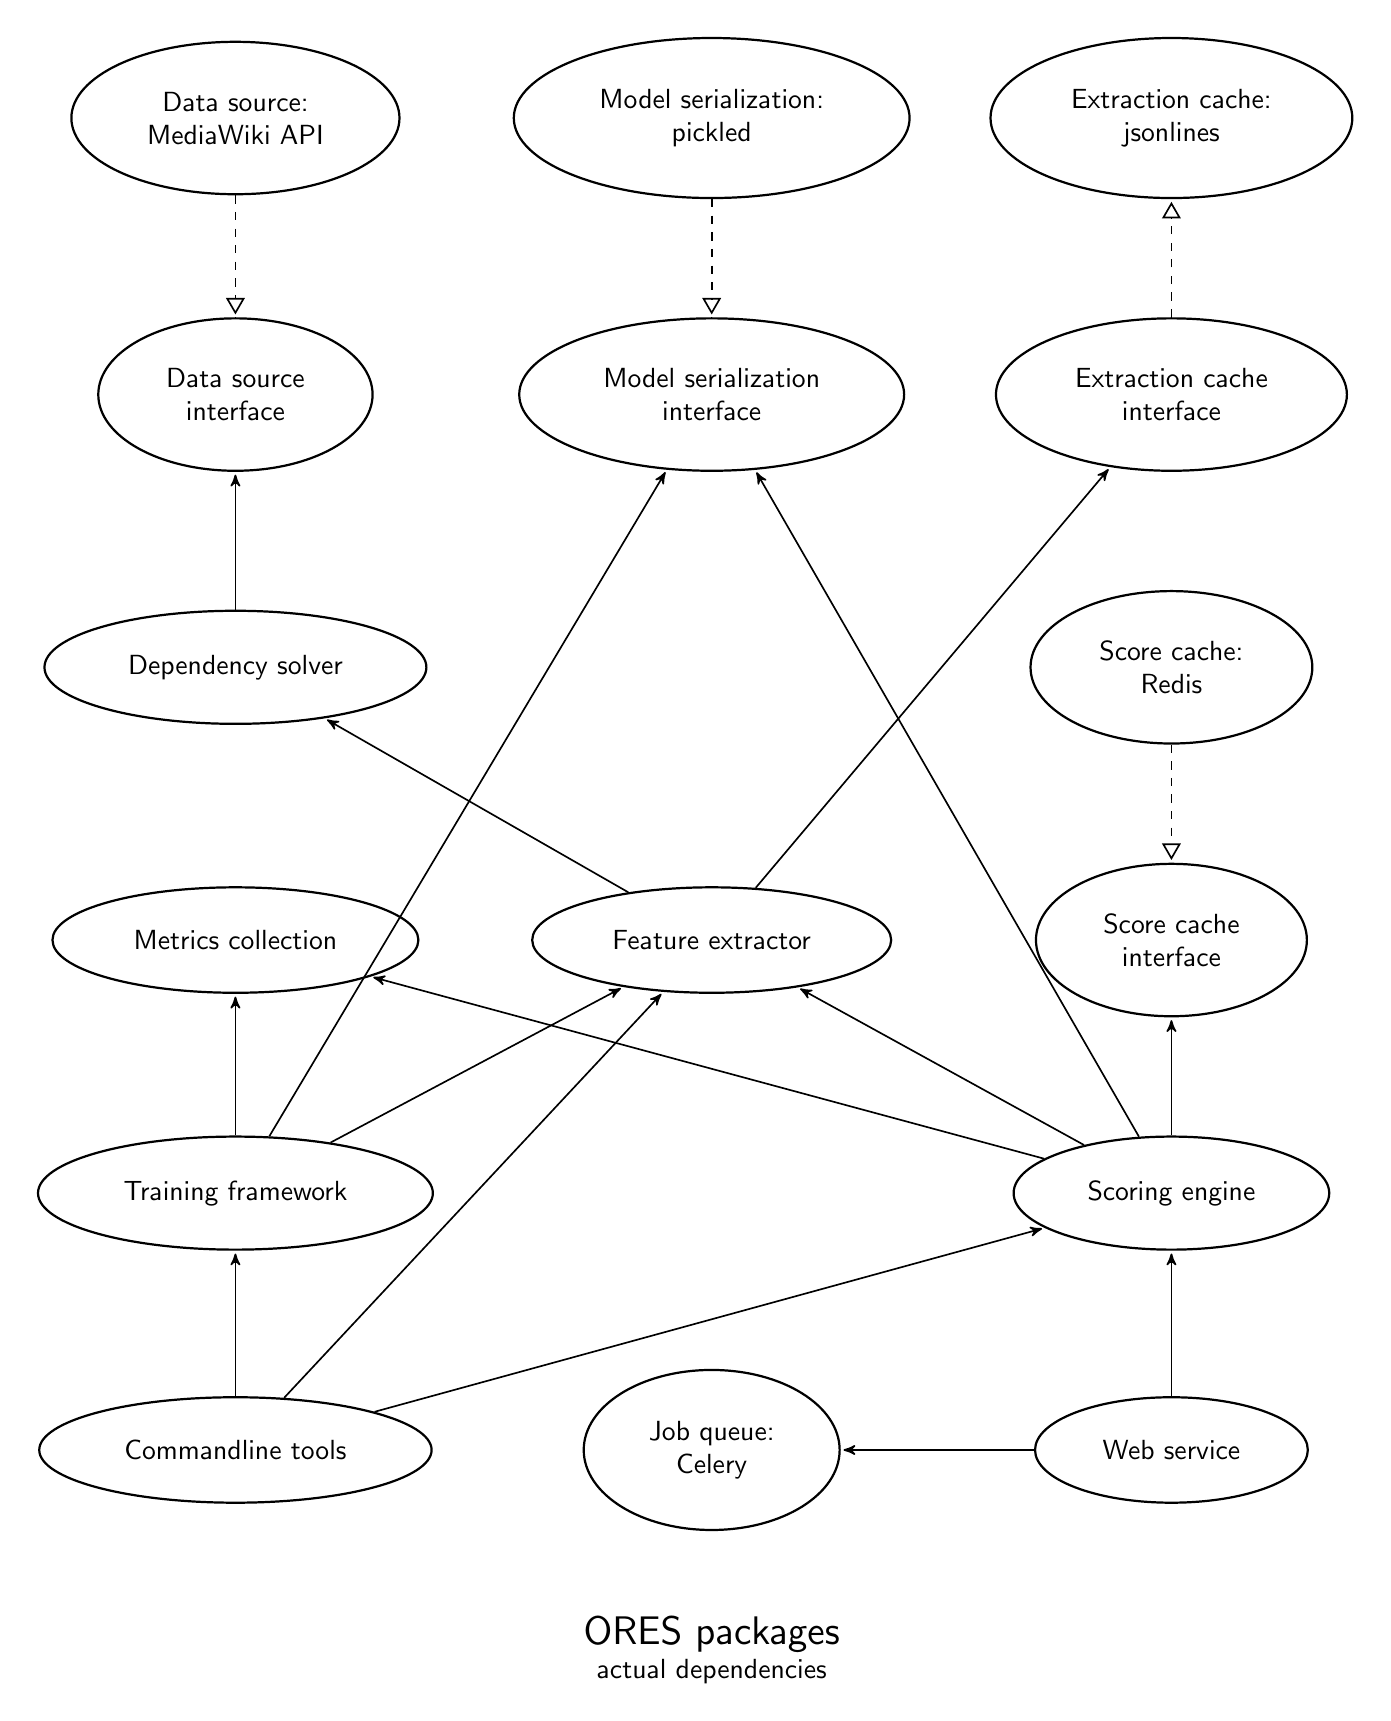
\begin{tikzpicture}[
  font=\sffamily,
  every matrix/.style={ampersand replacement=\&, column sep=1cm, row sep=1.5cm, fill=white},
  package/.style={draw, ellipse, thick, inner sep=1em},
  depends/.style={->, >=stealth', shorten >=1pt, semithick, font=\sffamily\footnotesize},
  realization/.style={->, dashed, >=open triangle 60, shorten >=1pt, semithick, font=\sffamily\footnotesize},
  line/.style={-, semithick, font=\sffamily\footnotesize},
  every node/.style={align=center}]

  % Position the nodes using a matrix layout
  \matrix{
    \node[package] (datasource-mw) {Data source: \\ MediaWiki API};
      \& \node[package] (serialization) {Model serialization: \\ pickled};
        \& \node[package] (extraction-cache-jsonlines) {Extraction cache: \\ jsonlines}; \\
    \node[package] (datasource-interface) {Data source \\ interface};
      \& \node[package] (serialization-interface) {Model serialization \\ interface};
        \& \node[package] (extraction-cache-interface) {Extraction cache \\ interface}; \\
    \node[package] (dependency) {Dependency solver};
          \& \& \node[package] (score-cache) {Score cache: \\ Redis}; \\
    \node[package] (metrics) {Metrics collection};
      \& \node[package] (extractor) {Feature extractor};
        \& \node[package] (score-cache-interface) {Score cache \\ interface}; \\
    \node[package] (training) {Training framework};
        \& \& \node[package] (scoring) {Scoring engine}; \\
    \node[package] (commandline) {Commandline tools};
        \& \node[package] (jobs) {Job queue: \\ Celery};
          \& \node[package] (webservice) {Web service}; \\
  };
  \draw[realization] (extraction-cache-interface) -- (extraction-cache-jsonlines);
  \draw[depends] (extractor) -- (extraction-cache-interface);
  \draw[depends] (extractor) -- (dependency);
  \draw[depends] (dependency) -- (datasource-interface);
  \draw[realization] (datasource-mw) -- (datasource-interface);
  \draw[depends] (commandline) -- (extractor);
  \draw[depends] (commandline) -- (training);
  \draw[depends] (commandline) -- (scoring);
  \draw[realization] (score-cache) -- (score-cache-interface);
  \draw[depends] (training) -- (extractor);
  \draw[depends] (training) -- (serialization-interface);
  \draw[depends] (training) -- (metrics);
  \draw[depends] (scoring) -- (serialization-interface);
  \draw[depends] (scoring) -- (score-cache-interface);
  \draw[realization] (serialization) -- (serialization-interface);
  \draw[depends] (webservice) -- (jobs);
  \draw[depends] (webservice) -- (scoring);
  \draw[depends] (scoring) -- (extractor);
  \draw[depends] (scoring) -- (metrics);

  \node [below=2cm, align=flush center] at (jobs)
  {\Large ORES packages \\ \normalsize actual dependencies};

\end{tikzpicture}
\end{adjustwidth}
\end{document}
